\chapter{Algorithm Concepts }
\label{sec:algorithm_concepts}

This chapter explains the concepts of the chosen algorithms for the offline global path planner and the path generation around an object in greater detail.

\section{Offline Global Path Planning Algorithm}

RRT* is a variation of the basic rapidly-exploring random tree algorithm as described in \citealp{Karaman2011}. Similiar to its predecessor, the algorithm is able to search high-dimensional configuration spaces by randomly building a tree starting from an initial state. With two further rewiring steps, the algorithm is asymptotically optimal. The following section will consider this offline global path planning algorithm step by step.

\subsection{RRT* Algorithm}
\label{(sec: rrt*)}

In Figure \ref{pics:rrt1}, a partially constructed tree is spreading from a starting configuration into the obstacle-free workspace. Furthermore, a goal state within a specific threshold area is defined. The red circles represent states, which consists of informations
 on their positions. \\

\begin{figure} [h]
	\centering
	\includegraphics[width=1\textwidth]{images/rrt1.png}
	\caption{A new node (black) is being added to the tree.}
	\label{pics:rrt1}
\end{figure}

In a first step, a random state on the map gets sampled. Control is applied from the inherent nearest state to get closer to the sample. In this case, the stepsize is added in the direction of the sample in order to generate a new state. If this connection does not intersect an obstacle, the new state is added to the tree. Otherwise, the current iteration terminates and the process starts from the beginning again by sampling a new configuration. In a further step, new possible parents within a defined neighbourhood radius are considered for the new state. A rewiring is performed, if the new connection is collision-free and results in a path with minimum cost. Thus the current edge gets replaced in order to still maintain a tree structure. Figure \ref{pics:rrt2} shows an example of this process. In Figure \ref{pics:rrt3}, the final rewiring step is taking place. Edges are created from the new state to its possible children vertices, if the path through the new states results in a lower cost than the path through the current parent of the children. At this point, the current iteration is completed and the process starts over again. The procedure is repeated, until a feasible path from the initial to the goal configuration is found (see Figure \ref{pics:rrt4}). Since RRT* is an asymptotically optimal path planning algorithm, this solution gets updated with further iterations.      

\begin{figure} [h]
	\centering
	\includegraphics[width=1\textwidth]{images/rrt2.png}
	\caption{Searching for new parent nodes: a) potential states and b) rewiring  }
	\label{pics:rrt2}
\end{figure}

\begin{figure} [h]
	\centering
	\includegraphics[width=1\textwidth]{images/rrt3.png}
	\caption{Searching for new children nodes: c) potential states and d) rewiring  }
	\label{pics:rrt3}
\end{figure}

\begin{figure} [h]
	\centering
	\includegraphics[width=1\textwidth]{images/rrt4.png}
	\caption{A feasible path between start and goal state.}
	\label{pics:rrt4}
\end{figure}
   
\subsubsection{Search Radius}

The search radius $r_{Search}$ is a non-constant variable and is calculated with the following formula (Formula \ref{eq:radius}):

\begin{equation}
r_{Search} = min(\gamma_{RRT^{*}}(log(card(V))/card(V)^{1/d},\eta)  
\label{eq:radius}
\end{equation}

\begin{equation}
\gamma_{RRT^{*}}>(2(1+1/d))^{1/d}(\mu(X_{free})/\xi)^{1/d}
\label{eq:gamma}
\end{equation}

\begin{itemize}
	\item
	$\gamma_{RRT^{*}}$ is a constant and is chosen such the inequality (Formula \ref{eq:gamma}) is met. On the basis of a theorem, the fulfilment of this requirement results in the asymptotic optimality of the RRT* algorithm,
	\item
	$\mu(X_{free})$ defines the Lebesgue measure\footnote{Measure that associate objects in the euclidean space with their content (length, area, volume)  } of the obstacle-free space,
	\item
	$\xi$ is the volume of the unit sphere\footnote{Sphere with unit radius in d-dimensional space (length, circle, sphere)},
	\item
	$d$ is the dimension of the workspace,
	\item
	$\eta$ corresponds to the stepsize,
	\item
	$card(V)$ defines the current number of configurations available in the workspace.
\end{itemize}

\begin{figure} [h]
	\centering
	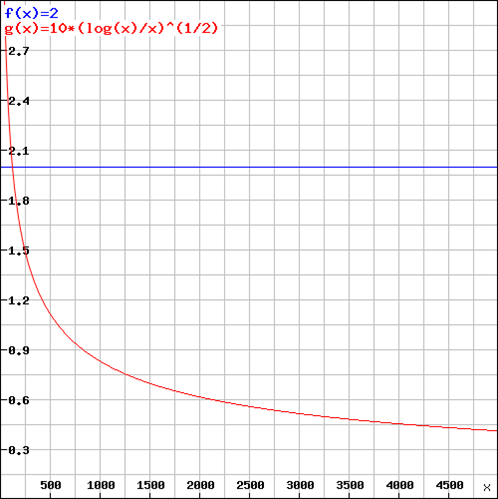
\includegraphics[width=0.75\textwidth]{images/radius.png}
	\caption{Plot of the search radius ($\eta=2,\gamma_{RRT^{*}}=10,d=2$, cardinality on the x- and radius on the y-axis)}
	\label{pics:radius}
\end{figure}

The search radius (see Formula \ref{eq:radius}) decreases logarithmically (see Figure \ref{pics:radius}) with the number of available configuration in the workspace. This choice is logical, since there are less required rewiring in a highly populated map needed. Furthermore, the computational effort of the collision-check function as well as the search of potential neighbours for the rewiring step gets released with a decrease of the search radius, which shortens the overall runtime of the algorithm.   

%\subsubsection{RRT* Pseudocode} 
%
%\begin{algorithm}[H]
%	\SetAlgoLined
%	$V \leftarrow {x_{init}}; E \leftarrow \emptyset$\;
%	\For{$i=1,...,n$}{		
%	$x_{rand} \leftarrow SampleFree$\;
%	$x_{nearest} \leftarrow Nearest(G=(V,E), x_{rand})$ \;
%	$x_{new} \leftarrow Steer(x_{nearest}, x_{rand})$ \; 	
%	\If{ObstacleFree($x_{x_{nearest}}, x_{x_{new}}$)} {
%		$X_{near} \leftarrow Near(G=(V,E), x_{new}, ...$
%		$... min\{\gamma_{RRT^{*}}(log(card(V))/card(V))^{1/d}, \eta)\}$\; 	
%		$V \leftarrow V \cup \{x_{new}\}$\;
%		$x_{min} \leftarrow x_{nearest}; c_{min} \leftarrow Cost(x_{nearest})+c(Line(x_{nearest}, x_{new}))$\;
%		\For{$x_{near} \in X_{near}$}{
%			\If{$CollisionFree(x_{near}, x_{new}) \land Cost(x_{near}) ...$
%			$...+c(Line(x_{near}, x_{new}))<c_{min}$}{
%				$x_{min} \leftarrow x_{near}; c_{min} \leftarrow Cost(x_{near})+c(Line(x_{near},x_{new}))$\;
%				}
%			$E \leftarrow E \cup \{(x_{min},x_{new})\}$\;
%			\For{$x_{near} \in X_{near}$}{
%				\If{$CollisionFree(x_{new}, x_{near}) \land Cost(x_{new})...$
%				$...+c(Line(x_{new}, x_{near})) < Cost(x_{near})$}{
%					$x_{parent} \leftarrow Parent(x_{near})$\;
%					$E \leftarrow (E \backslash \{(x_{parent},x_{near})\}) \cup \{(x_{new},x_{near})\}$\;
%					}			
%				}		
%			}	
%		}	
%	}
%	\textbf{return} $G=(V,E)$\;	
%\end{algorithm}

\section{Path Generation around an Object}

The second goal of the thesis is the generation of a feasible path around an underwater object. Summarized, the process works as follows. 

\begin{itemize}
\item
First N viewpoints around the object are manually calculated,
\item
all possible paths between them are generated,
\item
the order of visiting the viewpoints is figured out.

\end{itemize}

\subsection{Viewpoints Calculation}

The N viewpoints are set, such that the front camera of \textit{Scubo} is able to cover the whole object in one frame. Thus, the distance to the object was estimated with the horizontal and vertical angle of view of the camera. 

\subsection{Paths and Cost Matrix Generation}

In Figure \ref{pics:viewpoints_paths}, the viewpoint 1 is considered first. Feasible paths to other viewpoints are calculated using the RRT* algorithm (see Section \ref{(sec: rrt*)}). The costs, which are defined by the length from one viewpoint to another are stored in a $N\times N$ matrix (see Figure \ref{pics:viewpoints_paths}). 

\begin{figure} [h]
	\centering
	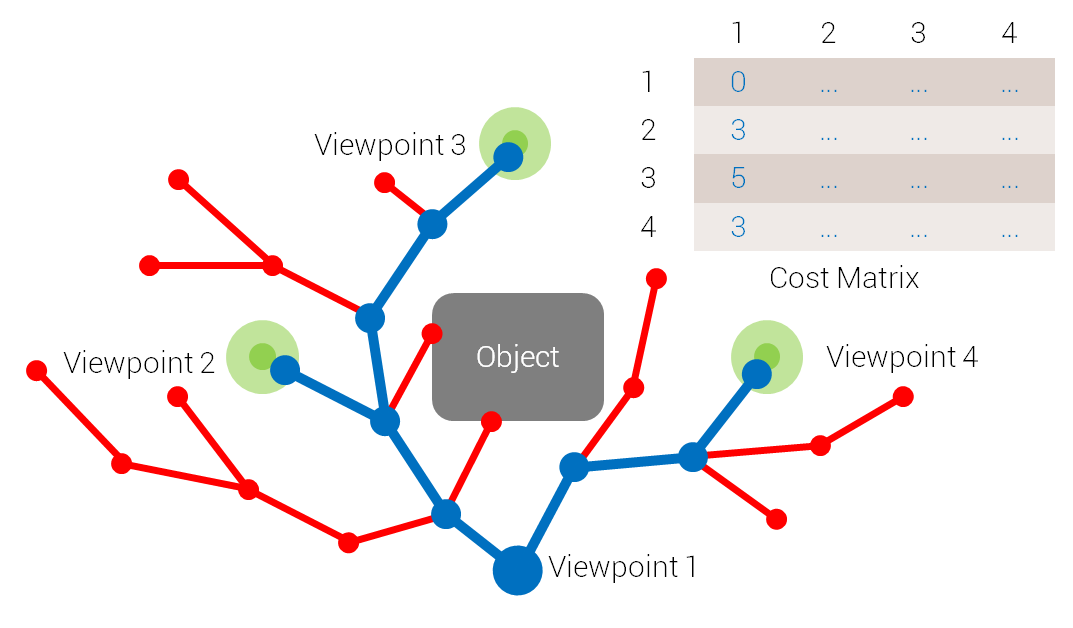
\includegraphics[width=1\textwidth]{images/cost_matrix_and_paths.png}
	\caption{Feasible paths to each viewpoint are calculated with the RRT* algorithm. The length of the paths are stored in a cost matrix.}
	\label{pics:viewpoints_paths}
\end{figure}

\subsection{Traveling Salesman Problem}

With the information about the viewpoints and the costs between them, the task of object scanning is reduced to a traveling salesman problem. The goal is to calculate the shortest possible route that visits each viewpoint exactly once and returns to the starting position. Large amount of heuristic and exact methods are able to approximate a solution of the problem. In the following, two of them are shortly introduced:

\begin{itemize}
	\item
	Greedy Algorithm: Makes the locally optimal choice at each stage. Thus, tends to find a local rather than a global optimum.
	\item
	Lin-Kernighan Heuristic (LKH): Randomly swapping pairs of sub-tours in order to generate a new more cost-optimal tour (see figure \ref{pics:lkh}). 
\end{itemize}

\begin{figure} [h]
	\centering
	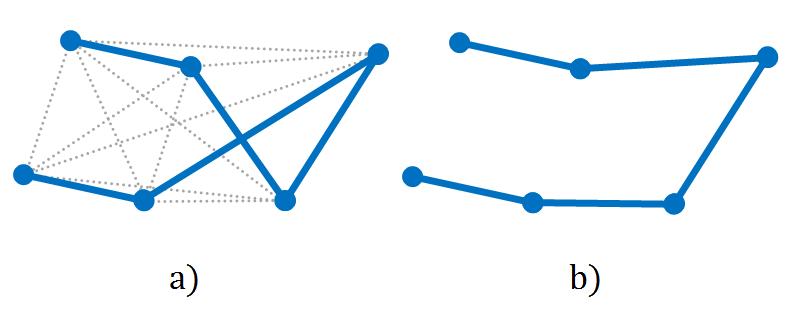
\includegraphics[width=0.6\textwidth]{images/LKH.png}
	\caption{Lin-Kernighan Heuristic: a) possible sub-tours in grey, b) optimal tour through eliminating cross-tours}
	\label{pics:lkh}
\end{figure}